% Start preamble
\documentclass[12pt,a4paper]{article}
\usepackage{geometry}
 \geometry{
 a4paper,
 total={170mm,257mm},
 left=20mm,
 top=20mm,
 }
\usepackage[utf8]{inputenc}
\usepackage[T1]{fontenc}
\usepackage[pdftex]{graphicx}
\graphicspath{{./}}
\usepackage{enumitem}
\usepackage{pdfpages}
\usepackage{hyperref}
\usepackage{tikz}
\usepackage{attachfile}
\usepackage{epstopdf}
\usepackage{array}
\usepackage{multirow}
\usepackage{multicol}
\usepackage{float}
%\usepackage[table]{xcolor,colorbl}
\setlength{\textwidth}{16cm}
\setlength{\oddsidemargin}{-0.5cm}
\setlength{\evensidemargin}{-0.5cm}
%\setlenght{\headsep}{0cm}
\setlength\parindent{0pt}
%\setlength{\extrarowheight}{3pt}
\usepackage{listings}
%\usepackage{xcolor}

\input{arduinoLanguage.tex}
%%%%%% Counting oppgaves %%%%%%
 \newcount\questnum \questnum=0
 \def\oppgave{
            \advance\questnum by 1
	    \ifthenelse{\questnum>0\AND \questnum<9}
	    {
                \vskip 1cm
		\textbf{Oppgave}\hskip 5pt\the\questnum \hfill \hfill(6p)
		\vskip 3pt
		\hrule
	\vskip 0.5cm}
	{
                \vskip 1cm
		\textbf{Oppgave}\hskip 5pt \the\questnum \hfill \hfill(12p)
		\vskip 3pt \hrule \vskip 0.5cm }

		}

% End preamble

\begin{document}
\title{TIF Pneumatikk 01}
\author{Faglærer: Fred-Olav Mosdal 90507684\\}
\maketitle
\oppgave{}%1
\vskip 2.5pt \begin{enumerate}
	\item Hva menes med overtrykk og undertrykk?
\vskip 2.5pt 
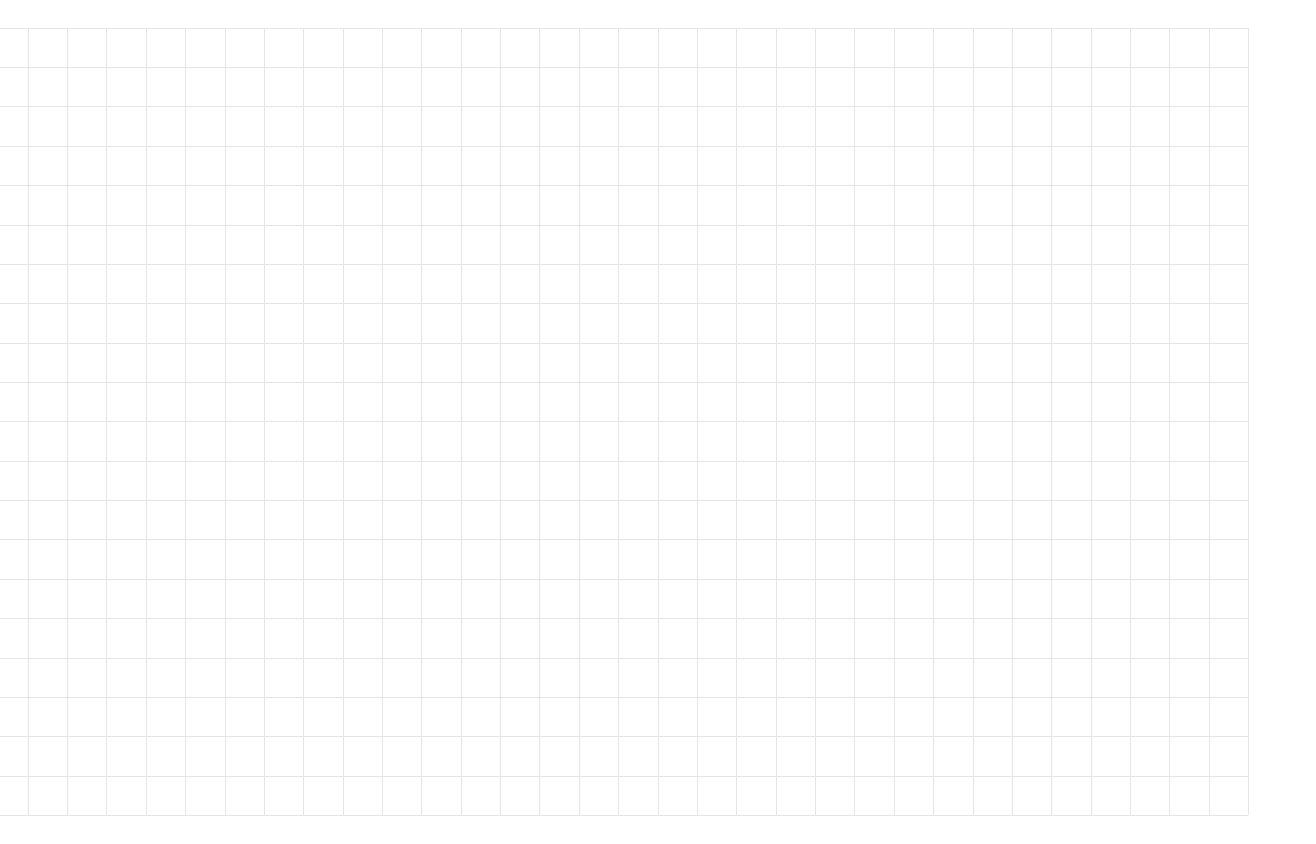
\begin{tikzpicture}
	\draw[step=0.5cm,gray!20,very thin]  grid (16,10) ;
\end{tikzpicture}
	\item Hva er et manometer?
\vskip 2.5pt 

\begin{tikzpicture}
	\draw[step=0.5cm,gray!20,very thin]  grid (16,2) ;
\end{tikzpicture}
\end{enumerate}


\vskip 2.5pt 
\newpage
\oppgave{}%2
\vskip 2.5pt\begin{enumerate}


\item Hva skjer i en tåkesmører?
\vskip 2.5pt 

\begin{tikzpicture}
	\draw[step=0.5cm,gray!20,very thin]  grid (16,3) ;
\end{tikzpicture}
\item Hvorfor benyttes luftfilter i et pneumatisk anlegg?
\vskip 2.5pt 

\begin{tikzpicture}
	\draw[step=0.5cm,gray!20,very thin]  grid (16,3) ;
\end{tikzpicture}
\end{enumerate}
\vskip 2.5pt
\oppgave{}%3
\vskip 2.5pt
\begin{enumerate}
\item Hva er en arbeidsenhet?
\\
\vskip 2.5pt 

\begin{tikzpicture}
	\draw[step=0.5cm,gray!20,very thin]  grid (16,3) ;
\end{tikzpicture}
\item Hva menes med plussretning og minusretning på en sylinder?
\\
\vskip 2.5pt 

\begin{tikzpicture}
	\draw[step=0.5cm,gray!20,very thin]  grid (16,3) ;
\end{tikzpicture}
\end{enumerate}
\newpage

\oppgave{}%4
\vskip 2.5pt 
\begin{enumerate}
\item Hvor mange funksjonelle stillinger har en 5/2-ventil?
\vskip 2.5pt 

\begin{tikzpicture}
	\draw[step=0.5cm,gray!20,very thin]  grid (16,3) ;
\end{tikzpicture}
\item Hvilket nummer har portene for a) tilkopling av trykkluft og b) utlufting (eksos)?
\vskip 2.5pt 

\begin{tikzpicture}
	\draw[step=0.5cm,gray!20,very thin]  grid (16,3) ;
\end{tikzpicture}
\end{enumerate}
\vskip 5pt 
\oppgave{}%5
\vskip 2.5pt 
Se på skjemategningen nedenfor. Forklar hva som skjer når vi betjener
trykknappen på retningsventilen.
\vskip 2.5pt 

\begin{tikzpicture}
	\draw[step=0.5cm,gray!20,very thin]  grid (9,9.5) ;
\end{tikzpicture}
\includegraphics[height=9cm]{../output/Pneumatikk03.png}\\

\begin{tikzpicture}
	\draw[step=0.5cm,gray!20,very thin]  grid (16,2.5) ;
\end{tikzpicture}
\vskip 2.5pt 
\newpage
\oppgave{}%6
\vskip 2.5pt 
Forklar hva de ulike komponentene på skjemaet gjør. Hva kalles denne samlingen av komponenter?\\
\includegraphics[width=1\textwidth]{../output/Pneumatikk01.png}\\
\vskip 2.5pt 

\begin{tikzpicture}
	\draw[step=0.5cm,gray!20,very thin]  grid (16,15) ;
\end{tikzpicture}
\oppgave{}%7
\vskip 2.5pt 
\includegraphics[width=0.5\textwidth]{../output/Pneumatikk02.png}\\
\vskip 5pt 
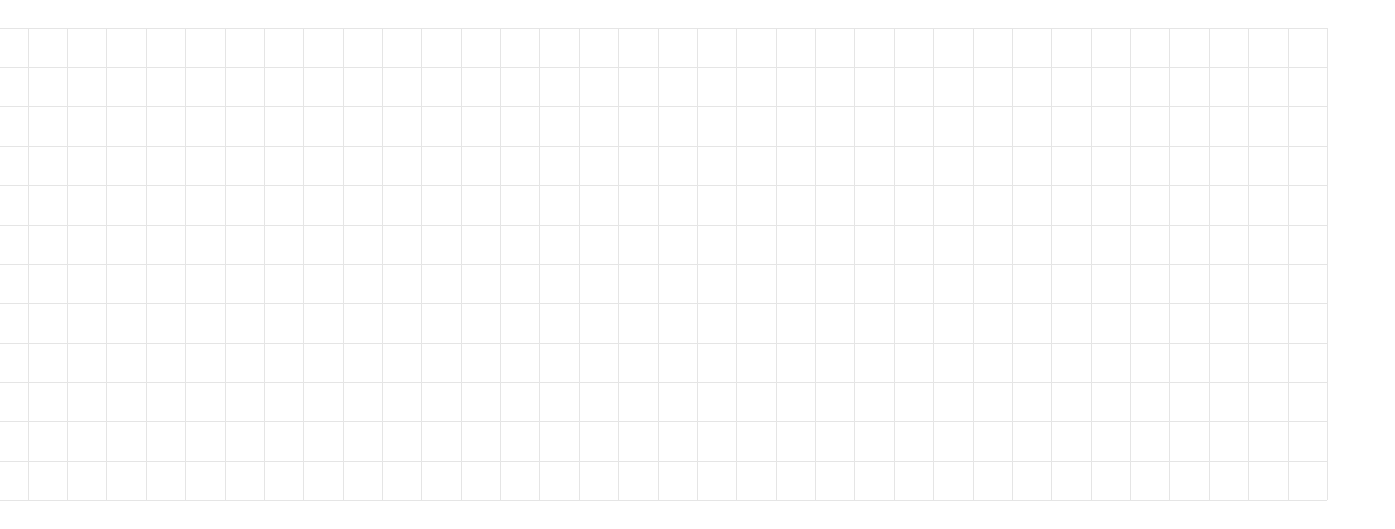
\begin{tikzpicture}
	\draw[step=0.5cm,gray!20,very thin]  grid (17,6) ;
\end{tikzpicture}
\vskip 2.5pt 
\oppgave{}%8
\vskip 2.5pt 
Hvor stor kraft får vi fra en sylinder med diameter på 45 mm når vi har et arbeidstrykk på 7 bar?
\vskip 5pt 
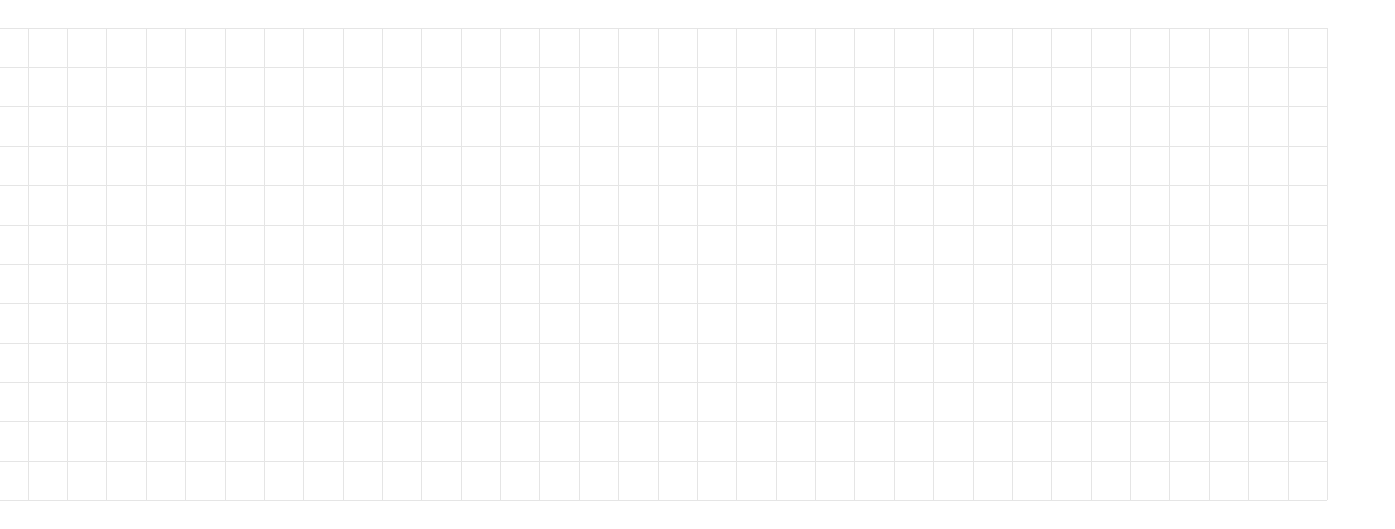
\begin{tikzpicture}
	\draw[step=0.5cm,gray!20,very thin]  grid (17,6) ;
\end{tikzpicture}
\vskip 2.5pt 
\newpage
\oppgave{}%9
\vskip 2.5pt 
\includegraphics[width=1\textwidth]{../output/Pneumatikk04.png}
\begin{enumerate}
	\item Hvilke pneumatiske komponenter vises i skjemaet?\\

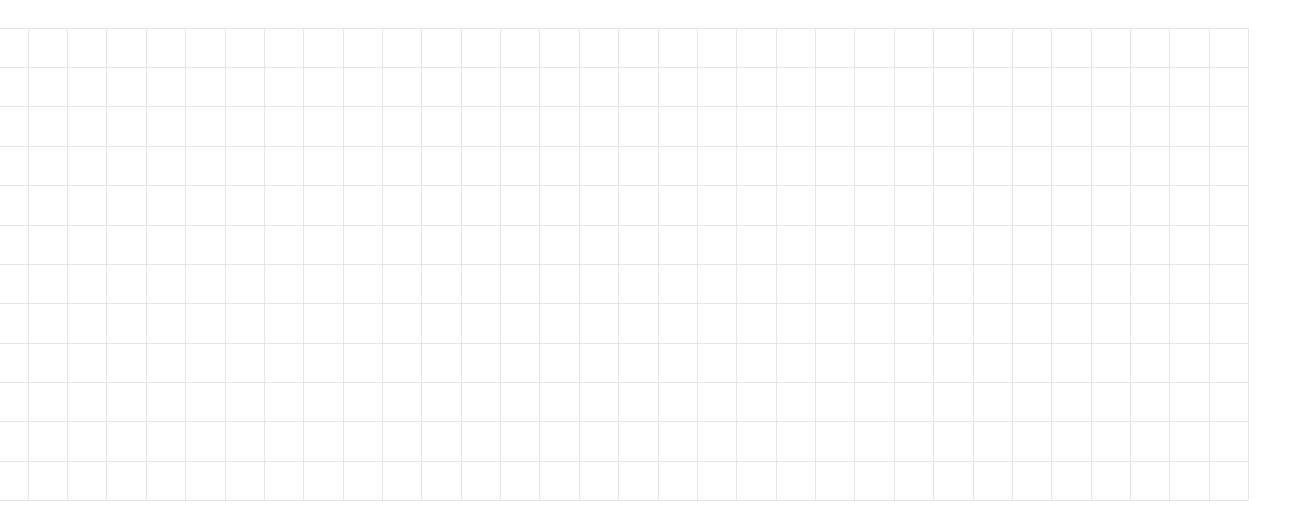
\begin{tikzpicture}
	\draw[step=0.5cm,gray!20,very thin]  grid (16,6) ;
\end{tikzpicture}
	\item Tegn koblingene som skal til for at hver av knappene skal styre arbeidsenheten i hver sin retning.
		\newpage
	\item Forklar hvordan kretsen virker.
\end{enumerate}
\vskip 5pt 
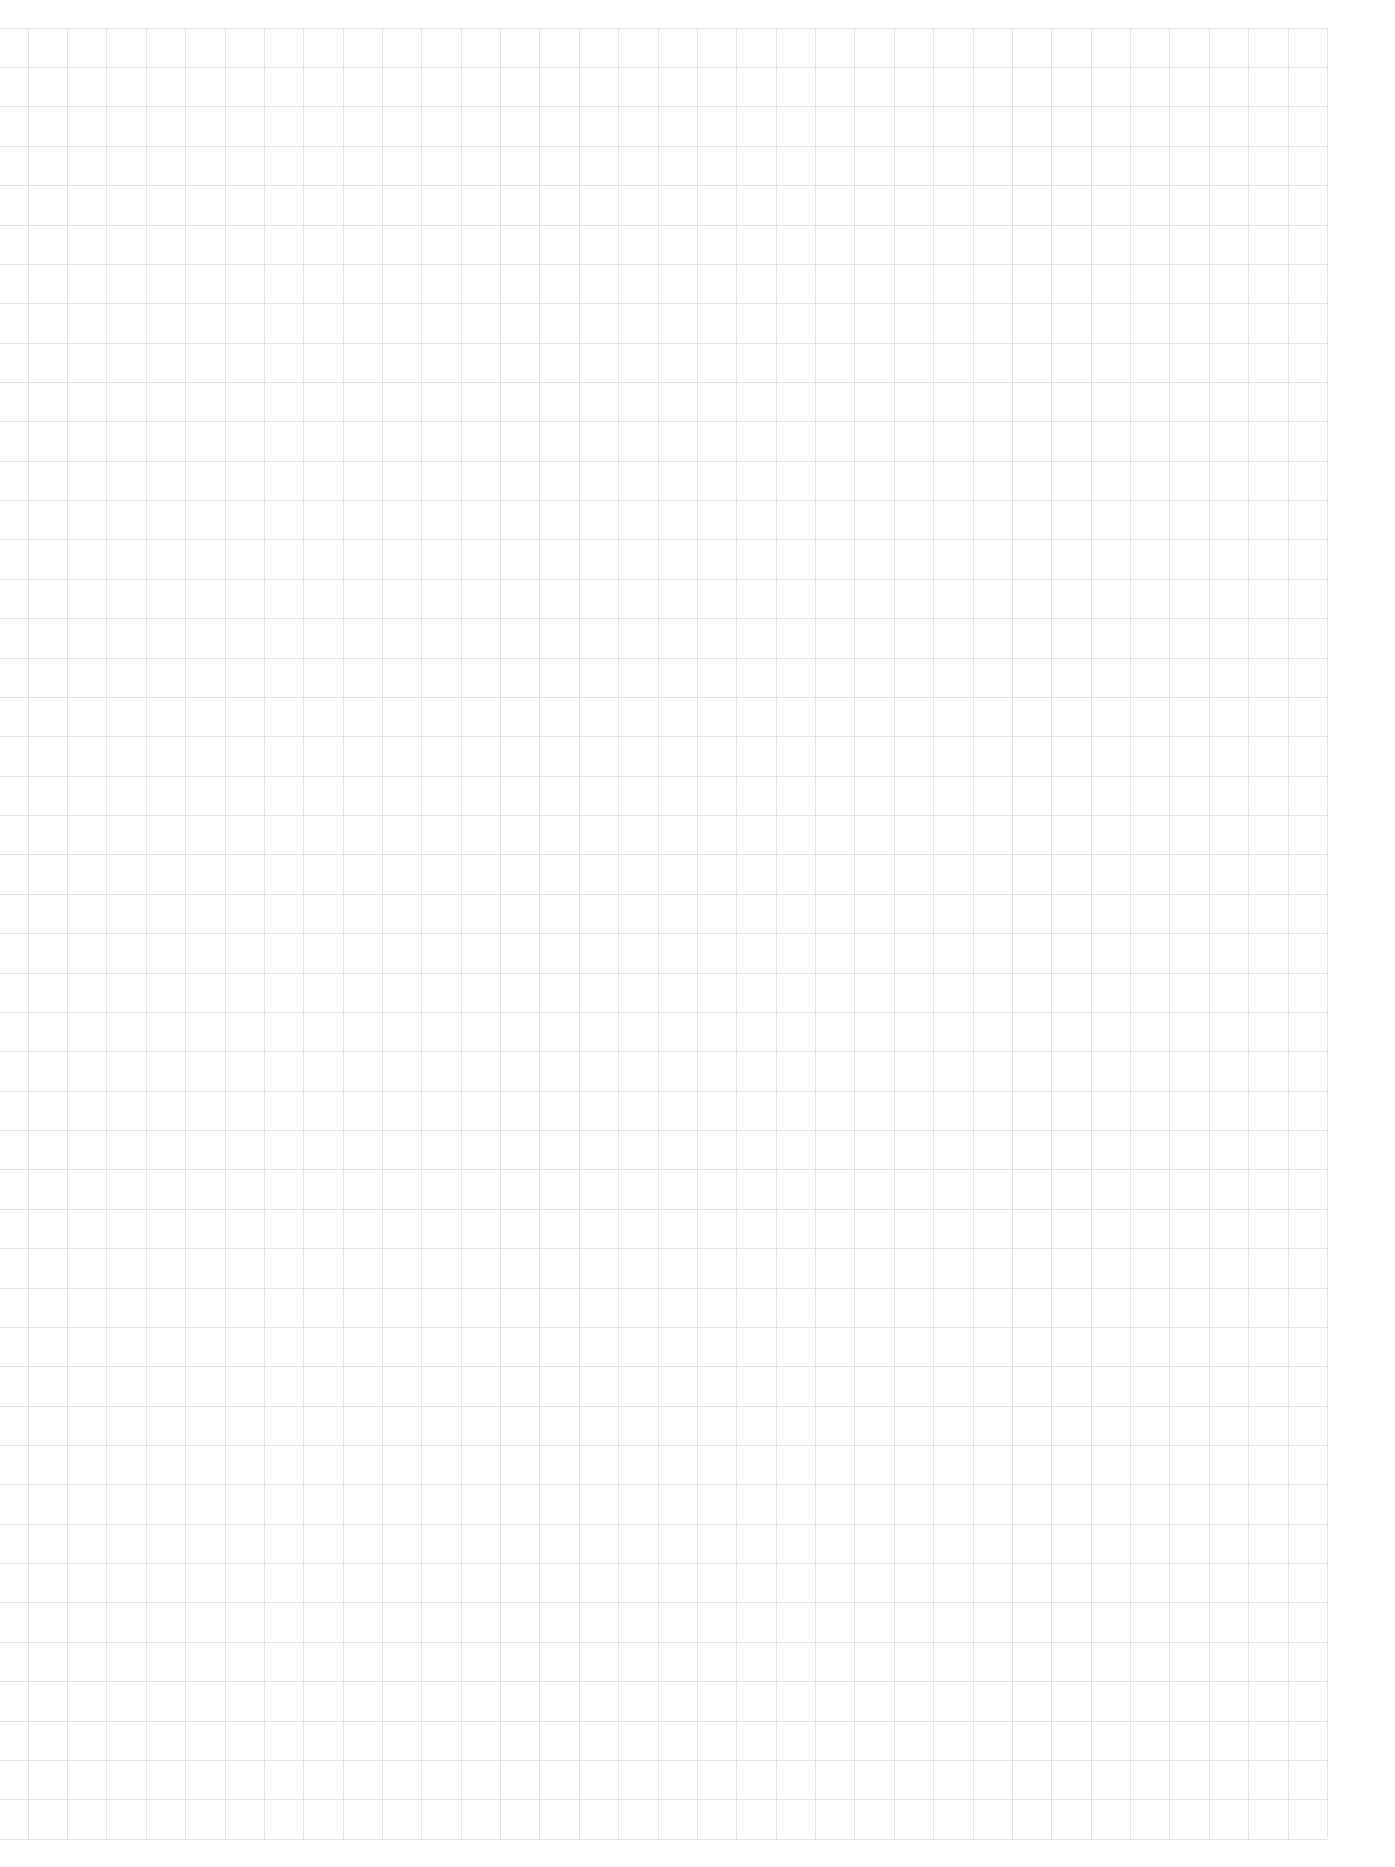
\begin{tikzpicture}
	\draw[step=0.5cm,gray!20,very thin]  grid (17,23) ;
\end{tikzpicture}
\vskip 2.5pt 
\newpage
\end{document}
